\section{Results}
\label{sec:results}

\subsection{Protocol}
\label{sec:protocol}

We compare four solvers. \sweep{} is the fixed-budget enumeration our renderer
shipped before this work: seed at $\rad(p)/s$, sweep a constant number of
neighbours, refine with Newton. \loose{} is the interval of
Theorem~\ref{thm:window} with the drift constant~\eqref{eq:drift} replaced by
$\lVert\delta\rVert$, isolating the contribution of
Section~\ref{sec:drift}. \ours{} is the full method. \textsc{Reference} is an
exhaustive scan at stride $1$ with no budget and no interval, terminating only on
the trivial certificate $\rad(q_n)\le \lVert p\rVert + nm$; it is independent of
the bound under test, so it can referee it.

The GPU numbers come from a standalone WebGPU harness that extracts the WGSL of
each solver generation directly from its source file, compiles it into an
identical compute kernel, and times a pass with GPU timestamp queries over a
$1200\times800$ point grid --- $0.96$\,Mpixel of solver work with no
rasterisation, no compositing, and no browser frame overhead in the measurement.
Reported values are the median of $9$ passes after $3$ warm-up passes, on an
Apple \texttt{\gpuAdapter} adapter. The CPU numbers come from a rasteriser that
mirrors the shader's compositing term for term, instrumented to count calls to
$\rad$; this is the only way to render an image with a solver that no longer
exists in the shader, and the only way to get a per-pixel work map.

All experiment scripts, the generated data, and every figure in this paper are in
the accompanying repository and reproduce with one command each.

\subsection{Cost}

% GENERATED by paper/tools/numbers.mjs
\begin{table}[t]
  \centering
  \small
  \caption{GPU pass time in milliseconds per megapixel of solver work, one
  full-screen family, Apple \texttt{metal-3}. \emph{Zoom} $0.15$ is a $6.7\times$
  zoom-out, where the index interval is widest. The last three rows are the hard
  cases of Section~\ref{sec:limits}: an offset close to the spacing, and the
  marginal drift $m=s$ itself. Bold marks the shipped method, not the row minimum:
  \loose{} is faster on the nonagon row, and loses ink globally
  (Table~\ref{tab:fidelity}).}
  \label{tab:gpu}
  \begin{tabular}{llrrr}
    \toprule
    Family & Zoom & \sweep{} & \loose{} & \ours{} \\
    \midrule
    Circle, rotation + offset & $1$ & $10.16$ & $0.33$ & $\mathbf{0.33}$ \\
    Circle, rotation + offset & $0.15$ & $15.47$ & $1.25$ & $\mathbf{1.05}$ \\
    Square, rotation & $1$ & $8.78$ & $0.26$ & $\mathbf{0.26}$ \\
    Square, rotation + offset & $0.15$ & $13.50$ & $0.85$ & $\mathbf{0.79}$ \\
    Square, offset only & $1$ & $0.92$ & $1.18$ & $\mathbf{0.20}$ \\
    Triangle, rotation & $1$ & $14.42$ & $0.52$ & $\mathbf{0.39}$ \\
    Triangle, rotation & $0.15$ & $20.12$ & $1.44$ & $\mathbf{0.92}$ \\
    Triangle, rotation + offset & $1$ & $16.97$ & $0.79$ & $\mathbf{0.52}$ \\
    Triangle, rotation + offset & $0.15$ & $27.85$ & $2.69$ & $\mathbf{1.64}$ \\
    Hexagon, rotation + offset & $0.15$ & $25.17$ & $2.23$ & $\mathbf{1.64}$ \\
    Nonagon, rotation + offset & $0.15$ & $23.40$ & $2.03$ & $\mathbf{2.16}$ \\
    \midrule
    Offset near spacing & $1$ & $43.32$ & $2.82$ & $\mathbf{1.57}$ \\
    Offset near spacing & $0.15$ & $46.73$ & $7.47$ & $\mathbf{5.44}$ \\
    Marginal drift $m=s$ & $1$ & $65.73$ & $30.47$ & $\mathbf{17.56}$ \\
    \bottomrule
  \end{tabular}
\end{table}

% GENERATED by paper/tools/numbers.mjs
\begin{table}[t]
  \centering
  \small
  \caption{Mean evaluations of $\rad$ per pixel, CPU rasterizer, and fraction of
  pixels differing from \textsc{Reference} by more than $8/255$. \ours{} agrees
  with brute force to within that tolerance at every pixel of all 7 scenes
  while doing less work than the exhaustive scan that defines the reference.}
  \label{tab:cost}
  \begin{tabular}{@{}lrrrr@{}}
    \toprule
    & \multicolumn{3}{c}{evaluations / pixel} & \ours{} \\
    \cmidrule(lr){2-4}
    Scene & \textsc{Ref.} & \sweep{} & \ours{} & differ \\
    \midrule
    Triangle, rotation & $21.9$ & $192.3$ & $7.6$ & $0.0\%$ \\
    Hexagon, rotation, zoomed out & $84.3$ & $180.0$ & $9.0$ & $0.0\%$ \\
    Triangle, translation & $19.2$ & $195.4$ & $11.0$ & $0.0\%$ \\
    Triangle, offset $=$ spacing & $46.0$ & $283.6$ & $11.0$ & $0.0\%$ \\
    Square, rotation + translation & $23.5$ & $201.9$ & $7.8$ & $0.0\%$ \\
    Deep zoom-out, small rotation & $43.5$ & $194.1$ & $\mathbf{7.5}$ & $0.0\%$ \\
    Two circle families, interfering & $49.5$ & $360.8$ & $11.1$ & $0.0\%$ \\
    \bottomrule
  \end{tabular}
\end{table}


Table~\ref{tab:gpu} gives GPU pass times. Across rotated settings \ours{} is
$\gpuSpeedLo$--$\gpuSpeedHi\times$ faster than \sweep{}. The absolute numbers are
what changed the tool: a single rotated triangle family went from
$\gpuTriRotOne$\,ms per megapixel --- alone, over budget for a $60$\,Hz frame ---
to $\gpuTriRotOneNew$\,ms, so a dozen layers now fit in the frame that one layer
used to miss. At $6.7\times$ zoom-out, where \sweep{} degrades to
$\gpuTriRotOffOut$\,ms, \ours{} costs $\gpuTriRotOffOutNew$\,ms. The
translation-only row shows Proposition~\ref{prop:closed} in isolation:
$\gpuSquareOld \to \gpuSquareClosed$\,ms, a $\gpuSquareClosedGain\times$ gain over
an already-cheap case, because the closed form needs no rotation and hence no
transcendentals.

Table~\ref{tab:cost} counts CPU evaluations of $\rad$ per pixel and, in the last
column, disagreement with the exhaustive reference. Two things stand out. \ours{}
costs $\costOursLo$--$\costOursHi$ evaluations per pixel where \sweep{} costs
$\costSweepLo$--$\costSweepHi$ --- a $\costVsSweepLo$--$\costVsSweepHi\times$
reduction in the quantity the shader actually pays for. And \ours{} is cheaper than
\textsc{Reference} itself, by $\costVsRefLo$--$\costVsRefHi\times$, despite
\textsc{Reference} being given a termination
certificate: the Lipschitz rule skips indices the exhaustive scan is obliged to
visit. Being faster than brute force while agreeing with it everywhere is the
cleanest summary of the method we can offer.

\subsection{Fidelity}

\begin{figure*}[t]
  \centering
  \begin{subfigure}{0.245\textwidth}
    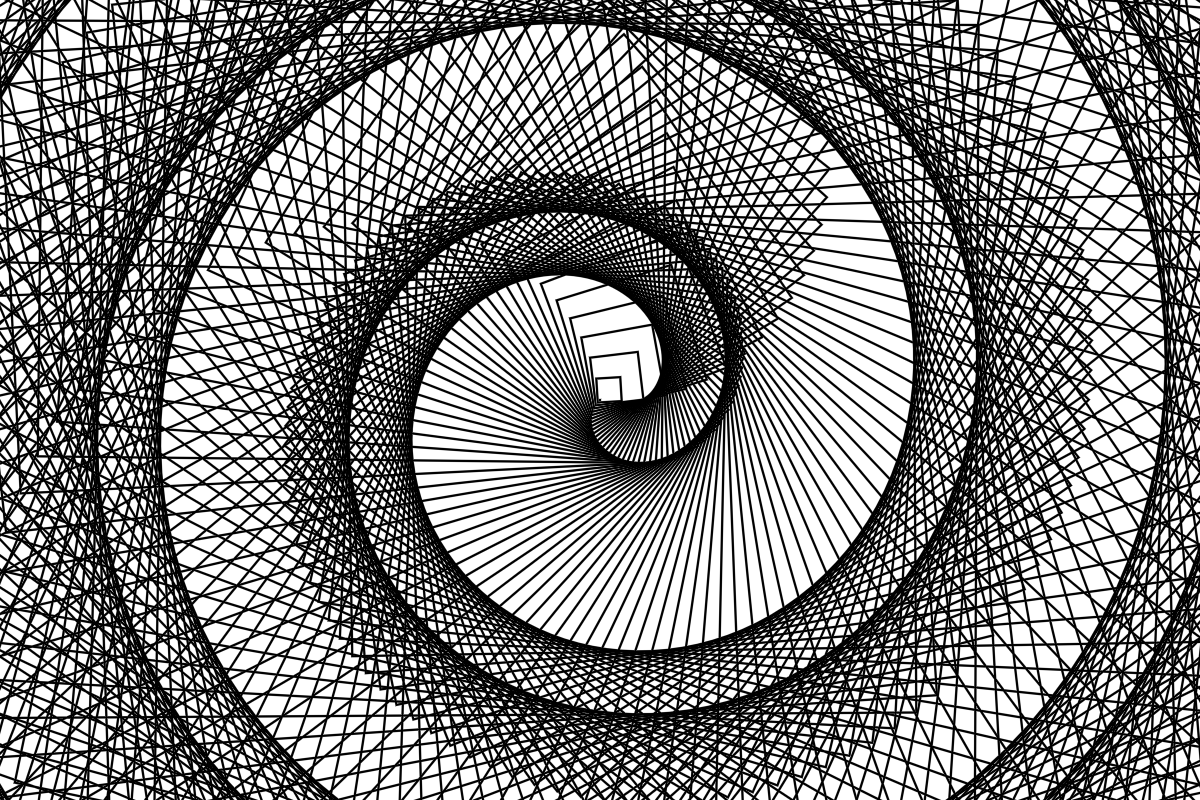
\includegraphics[width=\linewidth]{figures/artifact-holes-reference.png}
    \caption{\textsc{Reference}}
  \end{subfigure}\hfill
  \begin{subfigure}{0.245\textwidth}
    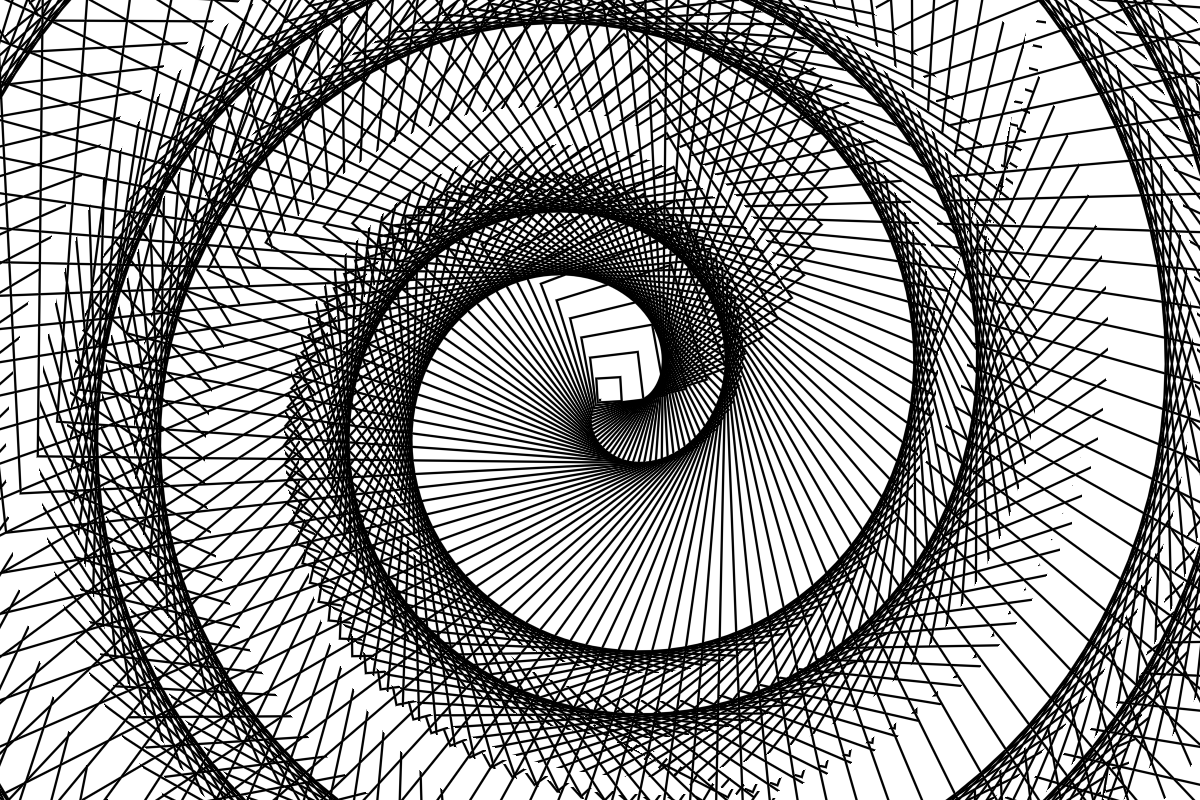
\includegraphics[width=\linewidth]{figures/artifact-holes-sweep.png}
    \caption{\sweep{}, $\artHolesSweepEv$ ev/px}
  \end{subfigure}\hfill
  \begin{subfigure}{0.245\textwidth}
    
\includegraphics[width=\linewidth]{figures/artifact-holes-sweep-drop.png}
    \caption{lost ink (magenta)}
  \end{subfigure}\hfill
  \begin{subfigure}{0.245\textwidth}
    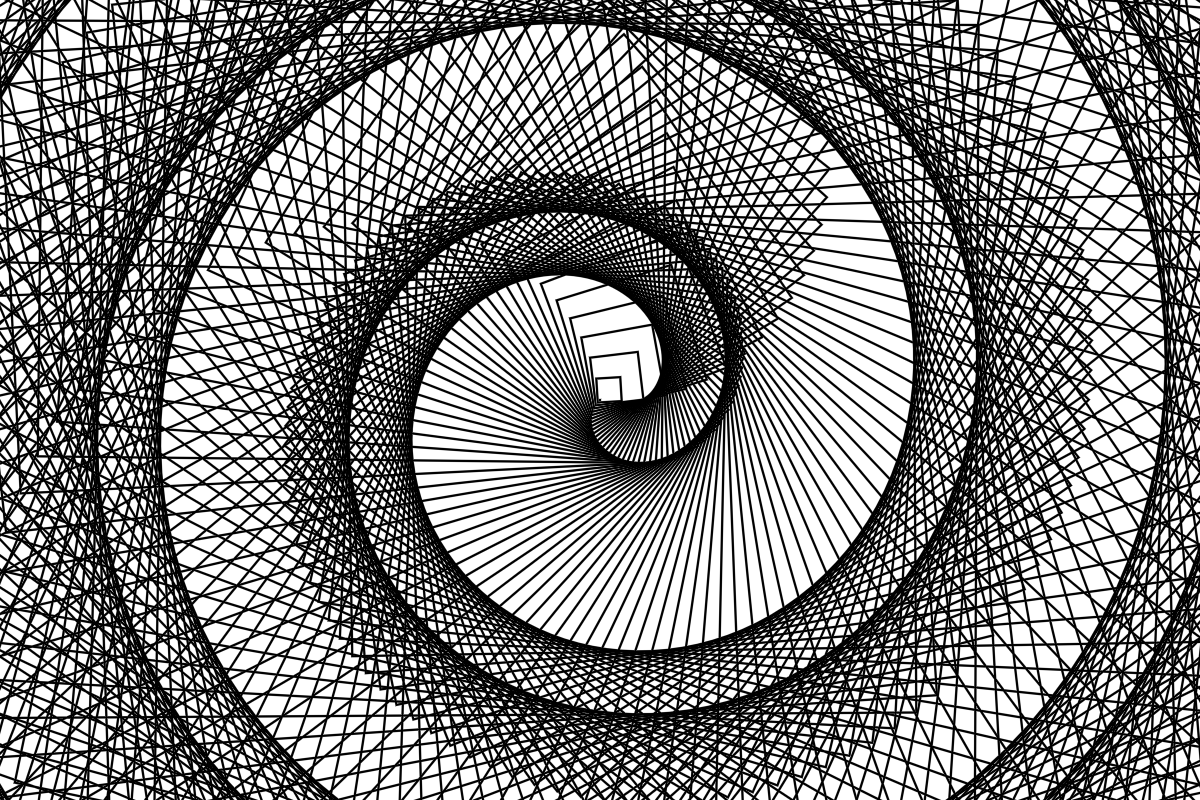
\includegraphics[width=\linewidth]{figures/artifact-holes-final.png}
    \caption{\ours{}, $\artHolesOursEv$ ev/px}
  \end{subfigure}
  \Description{Four wide panels of the same black-on-white field of walking
  hexagons, seen far from the family's centre: layers of finely woven arcs
  sweeping across the frame like drapery, with smooth dark bands between them.
  The first and fourth are identical. The second is visibly paler, with whole
  bands of the weave missing. The third is a pale grey copy of the pattern in
  which only the lost segments are drawn, in magenta, showing that the losses
  form broad coherent ribbons that follow the bands rather than scattered
  pixels.}
  \caption{Fixed enumeration deletes arcs, not pixels. The far field of a
  walking hexagon family whose drift aims at an edge --- almost a full spacing
  long, $\lVert\delta\rVert=0.95s$, while the support ratio stays at
  $\rad(-\delta)/s=0.82$; \sweep{} loses $\artHolesSweepDiff\%$ of the frame's
  pixels, and because the failure condition varies smoothly with $p$ the losses
  organise into coherent ribbons that read as missing bands. \ours{} is
  pixel-identical to the reference using $\artHolesSaving\times$ less work than
  \sweep{}. Insets in Figure~\ref{fig:insets}.}
  \label{fig:holes}
\end{figure*}

\begin{figure}[t]
  \centering
  \begin{subfigure}{0.32\linewidth}
    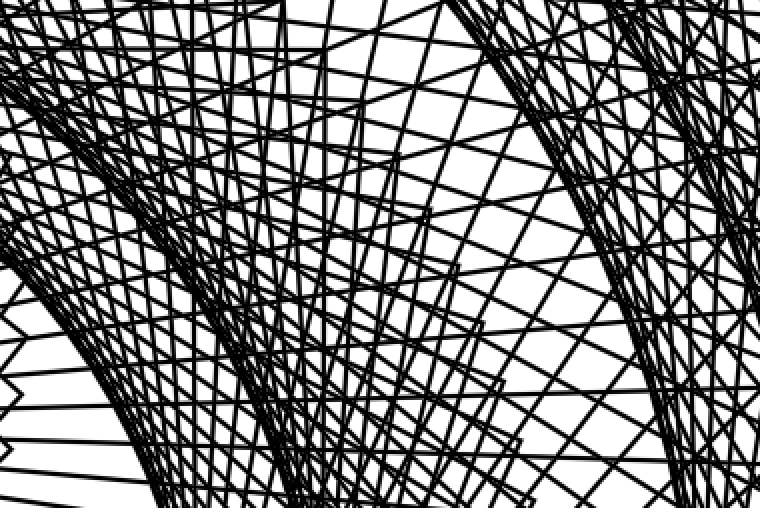
\includegraphics[width=\linewidth]{figures/inset-holes-reference.png}
    \caption{\textsc{Reference}}
  \end{subfigure}\hfill
  \begin{subfigure}{0.32\linewidth}
    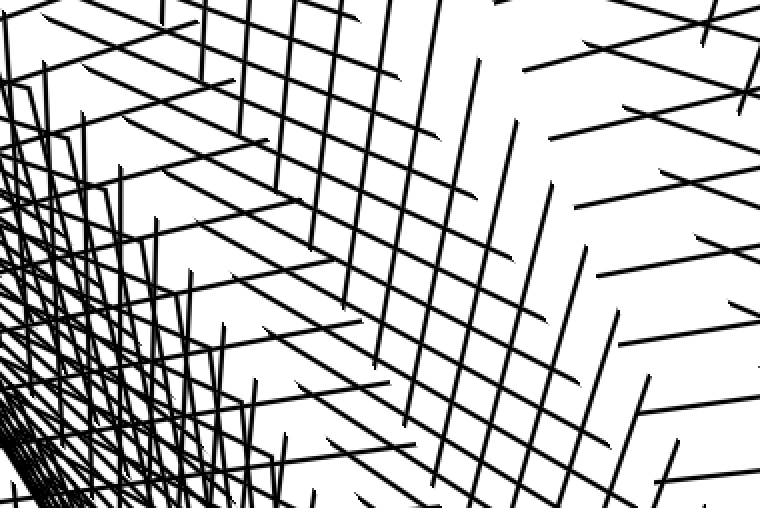
\includegraphics[width=\linewidth]{figures/inset-holes-sweep.png}
    \caption{\sweep{}}
  \end{subfigure}\hfill
  \begin{subfigure}{0.32\linewidth}
    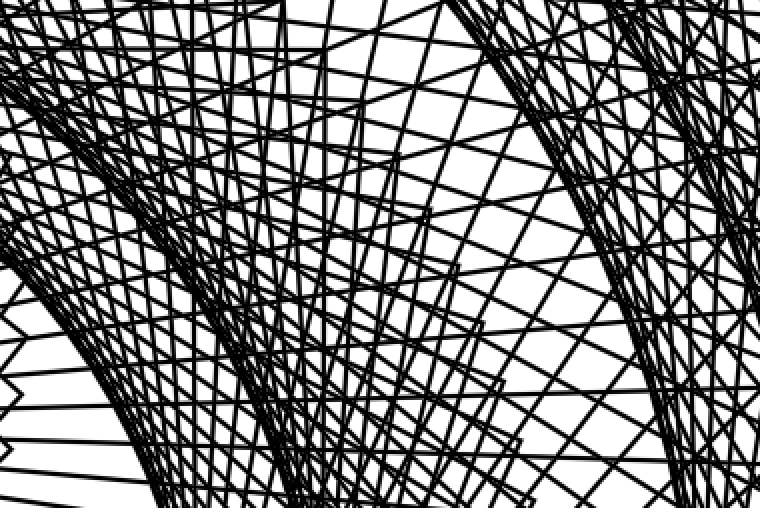
\includegraphics[width=\linewidth]{figures/inset-holes-final.png}
    \caption{\ours{}}
  \end{subfigure}
  \Description{Three magnified crops of a hatched pattern of crossing arcs. The
  first and third are identical and continuous. In the second, several arcs stop
  part-way across the crop and resume further on, leaving clean gaps.}
  \caption{$2\times$ crop of the worst region of Figure~\ref{fig:holes}. The
  missing ink is not noise; it is whole segments of whole rings, which is why the
  artifact survives supersampling and reads as a modelling error rather than an
  aliasing one.}
  \label{fig:insets}
\end{figure}

\begin{figure}[t]
  \centering
  \begin{subfigure}{0.32\linewidth}
    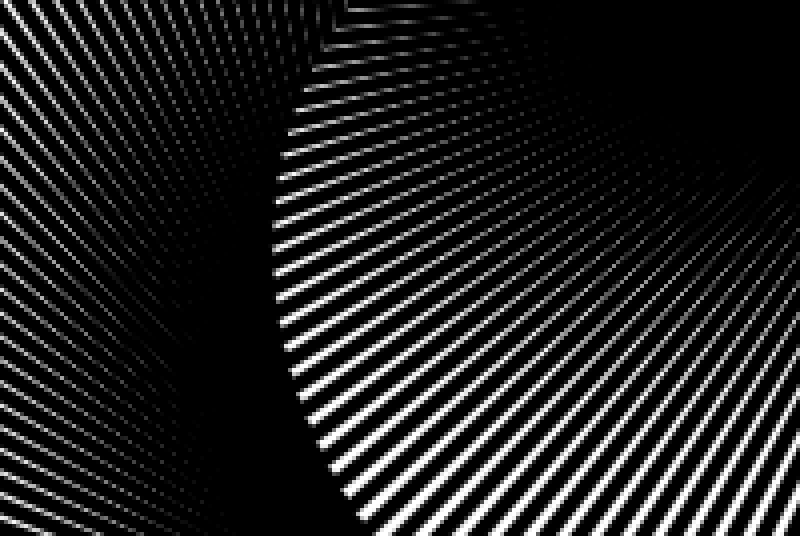
\includegraphics[width=\linewidth]{figures/inset-drift-reference.png}
    \caption{\textsc{Reference}}
  \end{subfigure}\hfill
  \begin{subfigure}{0.32\linewidth}
    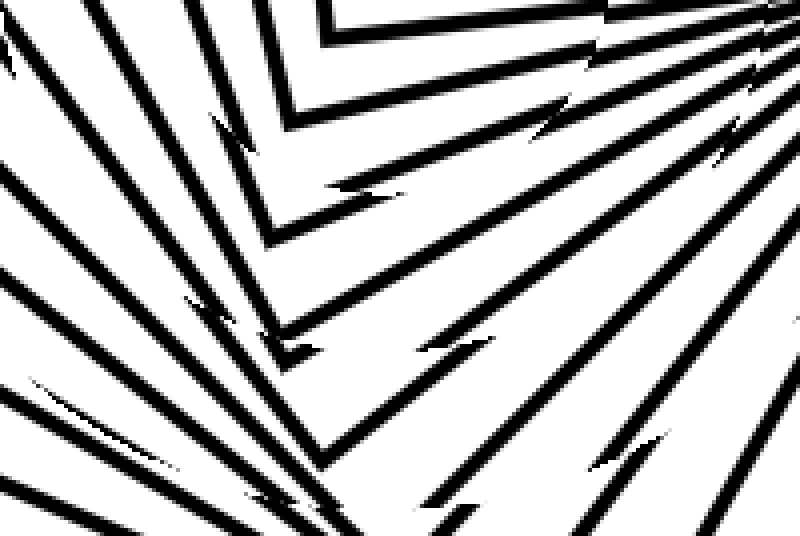
\includegraphics[width=\linewidth]{figures/inset-drift-window1.png}
    \caption{\loose{}}
  \end{subfigure}\hfill
  \begin{subfigure}{0.32\linewidth}
    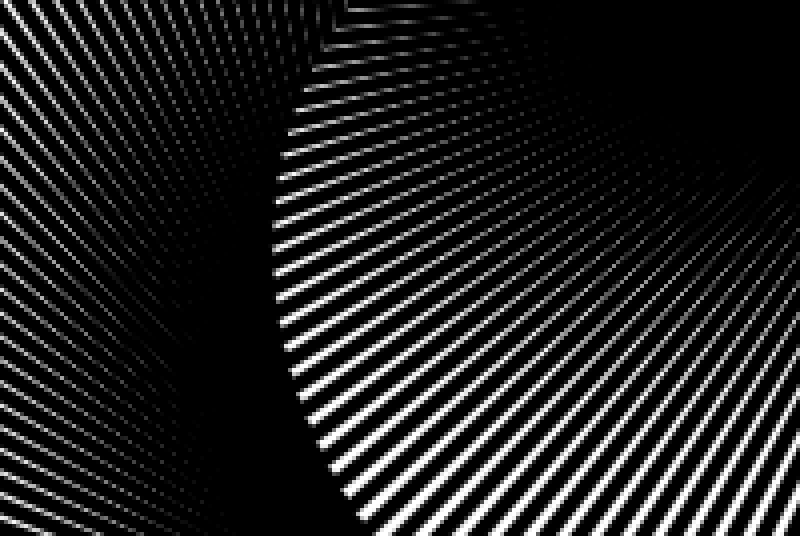
\includegraphics[width=\linewidth]{figures/inset-drift-final.png}
    \caption{\ours{}}
  \end{subfigure}
  \Description{Three magnified crops of a fan of straight strokes on black. The
  first and third match. The second has lost roughly two thirds of the strokes
  uniformly, so it reads as a sparser fan rather than a damaged one.}
  \caption{A loose drift constant is worse than a slow solver. \loose{} differs
  from~\eqref{eq:drift} only by using $\lVert\delta\rVert$ in place of
  $\rad(-\delta)$. That is enough to declare this setting's interval too wide to
  scan, so it subsamples: ink drops from $\artDriftRefInk$ to
  $\artDriftLooseInk$ and $\artDriftLooseDiff\%$ of pixels change. The exact
  constant keeps the interval finite and the pattern intact.}
  \label{fig:drift}
\end{figure}

We swept $\fidSettings$ parameter settings --- six shapes $\times$ spacings from
$1$ to $120$ $\times$ offsets $\times$ rotations $\times$ six zoom levels ---
and compared every solver against \textsc{Reference} at $512$ quasi-random points
each, classifying each point as agreeing, having lost ink, or having invented it.
Settings where the exhaustive reference would need more than $10^5$ evaluations
per point are counted and excluded rather than measured. Results in
Table~\ref{tab:fidelity}.

\begin{table}[t]
  \centering
  \small
  \caption{Ink lost against \textsc{Reference} over $\fidSettings$ settings.
  \emph{In interval} restricts to points where Theorem~\ref{thm:window}'s interval
  fits the budget, so exactness is claimed; \emph{legible} restricts to the
  $\fidLegible$ settings whose exact field is under $70\%$ ink, i.e. where a
  pattern is still visible. No solver ever invented ink, since all three minimise
  over a subset of $\N_0$.}
  \label{tab:fidelity}
  \begin{tabular}{lccc}
    \toprule
    & \sweep{} & \loose{} & \ours{} \\
    \midrule
    settings with holes            & $\fidSweepHoles$ & $\fidLooseHoles$ & $\fidOursHoles$ \\
    worst ink lost                 & $\fidSweepWorst\%$ & $\fidLooseWorst\%$ & $\fidOursWorst\%$ \\
    \midrule
    \emph{in interval}: settings   & $\fidSweepEnvelopeHoles$ & $\fidLooseEnvelopeHoles$ & $\mathbf{0}$ \\
    \emph{in interval}: worst      & $\fidSweepEnvelopeWorst\%$ & $\fidLooseWorst\%$ & $\mathbf{0.0\%}$ \\
    \midrule
    \emph{legible}: settings       & $\fidSweepLegibleHoles$ & $0$ & $\mathbf{0}$ \\
    \emph{legible}: worst          & $\fidSweepLegibleWorst\%$ & $0.0\%$ & $\mathbf{0.0\%}$ \\
    \bottomrule
  \end{tabular}
\end{table}

The row that matters is the third block. Wherever the proven interval fits the
budget --- the regime in which Theorem~\ref{thm:window} claims exactness --- \ours{}
disagrees with brute force at zero points out of $\fidSettings$ settings, while
\sweep{} disagrees in $\fidSweepEnvelopeHoles$ settings and loses up to
$\fidSweepEnvelopeWorst\%$ of the ink, and \loose{} up to $\fidLooseWorst\%$. The
theorem is not doing bookkeeping; it is the difference between an image and a
damaged one.

The $\fidOursHoles$ settings where \ours{} does lose ink are all outside the
envelope, and all of them are saturated: every one has an exact ink fraction above
$70\%$. Across the $\fidLegible$ legible settings, \ours{} loses nothing anywhere.
That is the honest form of the claim: exact where it claims to be, and in
particular exact everywhere a user can see a pattern.

Figures~\ref{fig:holes} and~\ref{fig:insets} show what the \sweep{} column looks
like on one scene, and Figure~\ref{fig:drift} isolates the drift constant. The
GPU twin agrees with the CPU twin to \texttt{f32} precision at every point where
the interval fits the budget.

\subsection{Ablation}

% GENERATED by paper/tools/numbers.mjs
\begin{table}[t]
  \centering
  \small
  \caption{Time relative to the full method when one mechanism is removed
  ($3.84$\,Mpixel of solver work). Each column is a different family, chosen so
  that every mechanism has a column where it binds. Values below $1$ mean the
  mechanism costs time in that setting, which is the price of exactness
  elsewhere.}
  \label{tab:ablation}
  \begin{tabular}{lcccc}
    \toprule
     & \multicolumn{2}{c}{rotated} & \multicolumn{2}{c}{translated} \\
    \cmidrule(lr){2-3}\cmidrule(lr){4-5}
    Mechanism removed & tri. & hex.\ out & near $s$ & marginal \\
    \midrule
    Lipschitz skip (\S\ref{sec:skip}) & $2.03$ & $2.29$ & $3.12$ & $1.00$ \\
    Support fast paths (\S\ref{sec:walking}) & $1.31$ & $1.16$ & $1.00$ & $1.49$ \\
    Exact drift (\S\ref{sec:drift}) & $1.00$ & $1.00$ & $1.25$ & $1.00$ \\
    Polygon closed form (\S\ref{sec:closed}) & $0.97$ & $0.99$ & $0.98$ & $\mathbf{101.2}$ \\
    Carried rotation (\S\ref{sec:skip}) & $0.95$ & $0.91$ & $0.93$ & $1.01$ \\
    Accept early exit (\S\ref{sec:guard}) & $0.91$ & $0.91$ & $0.90$ & $1.04$ \\
    \bottomrule
  \end{tabular}
\end{table}


Table~\ref{tab:ablation} removes one mechanism at a time. The Lipschitz skip is
the largest single lever ($\ablSkipLo$--$\ablSkipHi\times$), and the polygon closed
form is decisive exactly where predicted: on the marginal drift it is worth
$\ablClosedMarginal\times$, because without it the scan must walk a $2^{16}$-wide
interval to find an answer that Proposition~\ref{prop:closed} reads off in one
comparison.

Two entries are below $1$: removing the carried rotation or the accept-early-exit
is $\ablCostLo$--$\ablCostHi\%$ \emph{faster} in these dense scenes, a wavefront-%
divergence effect. We keep both because they are what make sparse and mid-density
scenes cheap; the divergence reading, and why narrowing the interval rather than
exiting sooner is the productive lever on a GPU, are in the supplemental
material (\S S3).

\subsection{Where the guarantee ends}
\label{sec:limits}

\begin{figure}[t]
  \centering
  \begin{tikzpicture}
    \begin{axis}[paperaxis, height=5.6cm,
      xlabel={interval span (indices, $\log_2$ bins)},
      ylabel={exact ink fraction},
      xmode=log, log basis x=2,
      xmin=1.5, xmax=131072, ymin=0, ymax=1,
      legend style={at={(0.5,-0.44)}, anchor=north, draw=none, fill=none,
                    /tikz/every even column/.append style={column sep=0.5cm}},
      legend columns=3,
    ]
      \addplot[draw=none, fill=cool!12, forget plot] coordinates
        {(1024,0) (131072,0) (131072,1) (1024,1)} \closedcycle;
      \addplot[cool, very thick, mark=*, mark size=1.3pt]
        table [x=span, y=medianInk, col sep=comma] {data/saturation.csv};
      \addlegendentry{median}
      \addplot[warm, thick, mark=square*, mark size=1.1pt]
        table [x=span, y=q25, col sep=comma] {data/saturation.csv};
      \addlegendentry{lower quartile}
      \addplot[accent, thick, densely dashed]
        table [x=span, y=minInk, col sep=comma] {data/saturation.csv};
      \addlegendentry{minimum}
      \node[soft, font=\scriptsize, anchor=south east] at (rel axis cs: 0.995, 1.015)
        {beyond budget $B$};
      \node[anchor=north west, inner sep=1.5pt, fill=white, draw=soft, semithick]
        at (rel axis cs: 0.035, 0.95) {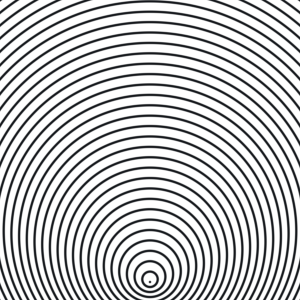
\includegraphics[width=1.35cm]{figures/inset-saturation-open.png}};
      \node[anchor=south east, inner sep=1.5pt, fill=white, draw=soft, semithick]
        at (rel axis cs: 0.90, 0.26) {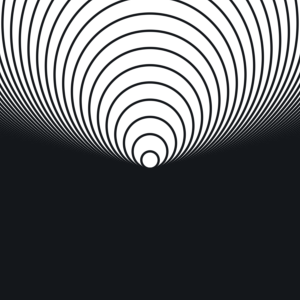
\includegraphics[width=1.35cm]{figures/inset-saturation-solid.png}};
    \end{axis}
  \end{tikzpicture}
  \Description{A line plot of exact ink fraction against interval span on a base-two
  logarithmic axis. Median and lower-quartile curves both rise monotonically from
  near zero at span two to about $0.9$ by span $2^{10}$, where a shaded region marks
  the budget and beyond which both stay high. A dashed minimum curve stays near zero
  until roughly span $2^{10}$ and then rises only to about $0.2$.}
  \caption{The interval is wide only where the pattern is already solid.
  $\satSettings$ settings, binned by the $90$th-percentile interval span, against
  the ink fraction of the exact field. Past the budget $B=\satBudget$ (shaded) the median
  setting is $\satMedianInk$ ink --- a nearly filled rectangle, where no point
  sample of the distance field is meaningful and the honest output is the filtered
  mean~\cite{Norton1982}. The insets are one walking circle family at both ends
  of the axis: a benign drift, whose pattern is open and whose interval is a few
  indices, and the near-marginal drift, where the interval explodes --- into a
  frame that is already solid ink. The dashed minimum is the honest caveat: sparse
  exceptions exist.}
  \label{fig:saturation}
\end{figure}

\begin{figure}[t]
  \centering
  \begin{subfigure}{0.32\linewidth}
    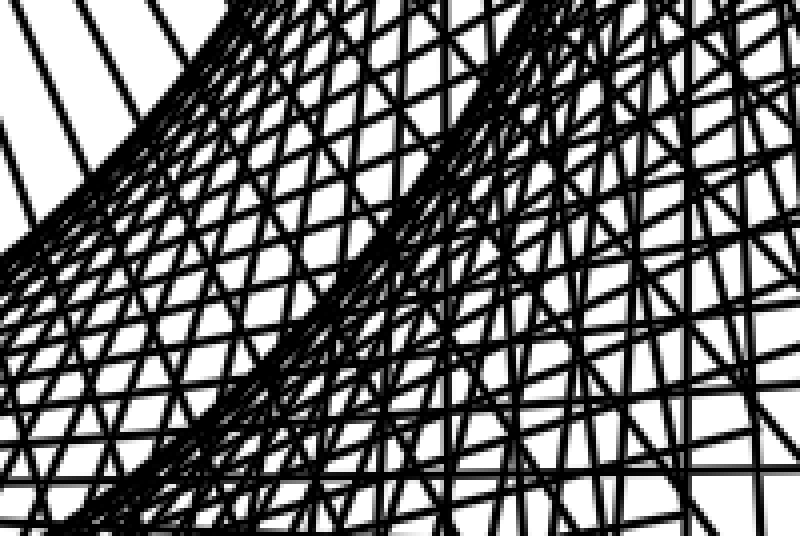
\includegraphics[width=\linewidth]{figures/inset-anchor-reference.png}
    \caption{exact}
  \end{subfigure}\hfill
  \begin{subfigure}{0.32\linewidth}
    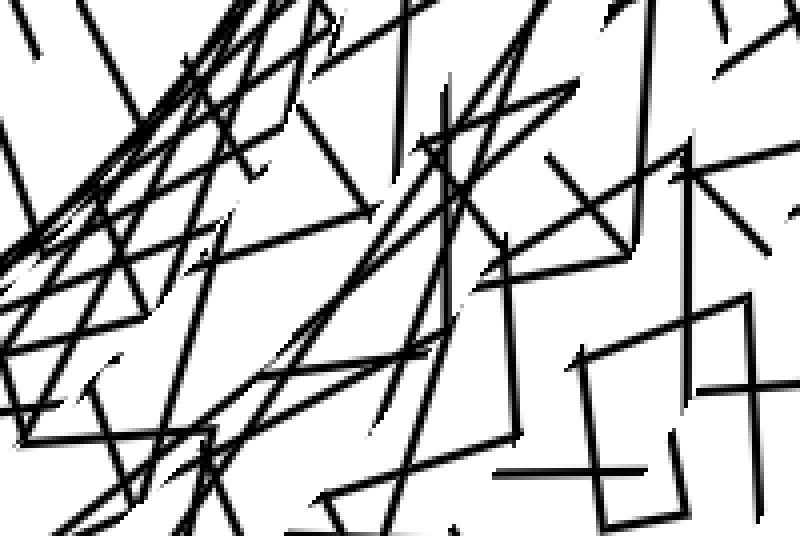
\includegraphics[width=\linewidth]{figures/inset-anchor-pixel-anchored.png}
    \caption{pixel-anchored}
  \end{subfigure}\hfill
  \begin{subfigure}{0.32\linewidth}
    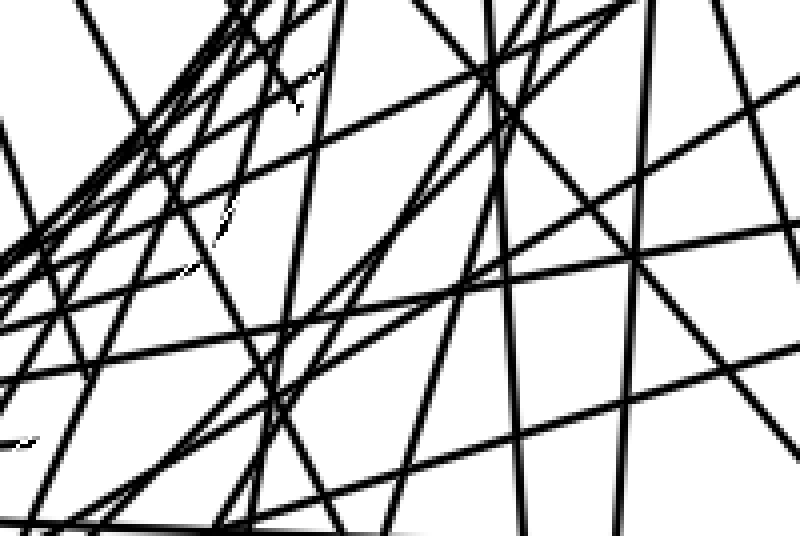
\includegraphics[width=\linewidth]{figures/inset-anchor-lattice-anchored.png}
    \caption{lattice-anchored}
  \end{subfigure}
  \Description{Three heavily magnified crops of a crosshatch of straight strokes.
  The first is a clean lattice of crossings. The second has broken into short
  disconnected dashes and hooks with no continuous line anywhere. The third is a
  clean lattice again, sparser than the first but with every stroke whole.}
  \caption{When you cannot be exact, be coherent. $4\times$ crops of one scene
  with the budget forced to $64$ so the stride engages while the field is still
  legible. Both subsamplings spend $\artAnchorEv$ evaluations per pixel and retain
  the same ink ($\artAnchorPixelInk$ vs $\artAnchorLatticeInk$ of the exact
  $\artAnchorRefInk$). Anchoring the stride to the pixel's own interval (centre) makes
  neighbouring pixels sample different rings, and the pattern shatters into dashes
  and hooks. Anchoring it to the global index lattice (right) makes them agree, and
  the same missing ink becomes a thinner family of whole straight lines --- a
  plausible pattern rather than a broken one. The two differ by one line of code.}
  \label{fig:anchor}
\end{figure}

Theorem~\ref{thm:window} gives an interval; it does not promise a small one. Two
questions follow: how often is it too wide to walk, and what happens then.

\emph{How often.} Over $\satSettings$ settings spanning the whole parameter space
our interface exposes, the interval fits the $B=\satBudget$ budget in $\satFitting$ of
them ($\satFittingPct\%$), and the widest fitting span we observed is
$\satWidestFitting$ --- so the budget is nearly exactly the right size, not an
arbitrary large number. In the remaining $\satStrided$ the interval exceeds the
budget. Every one of those has $m$ within a factor of $\satDriftRatioHi$ of $s$;
the wide-interval regime is precisely the near-marginal band, as the theory
predicts.

\emph{What the field looks like there.} Figure~\ref{fig:saturation} answers this
without needing an exhaustive reference, using the observation that any partial
scan takes a minimum over a subset and therefore \emph{over}-estimates $d$ and
\emph{under}-estimates ink: a measured ink fraction is a valid lower bound on the
true one. Ink rises monotonically with interval span, and past the budget the median
setting is $\satMedianInk$ ink. These are fields whose curves are far denser than
the pixel grid --- the regime where point sampling any distance field is
meaningless and the correct answer is a prefiltered
mean~\cite{Norton1982, Bruneton2012}. Only $\satStridedLegible$ settings
($\satStridedLegiblePct\%$ of the sweep) are both beyond the budget and legible.

\emph{What we lose there.} For those we cannot use the exhaustive reference, so we
compare against the same solver with $B$ raised to $131072$, which walks every
index inside the span cap at stride $1$. Over $\degChecked$ strided settings,
$\degWithDrop$ lose some ink; the mean loss is $\degMean\%$ and the worst is
$\degWorst\%$, in a setting whose exact field is $100\%$ ink. Restricted to the
$\degLegible$ legible ones the worst loss is $\degLegibleWorst\%$. We do not
claim correctness here and we do not claim a prefiltered mean; this is a genuine
limitation, confined to a $\satStridedLegiblePct\%$ band of parameter space, and it
is the obvious target for future work (Section~\ref{sec:future}).

\emph{What we do about it.} What we can control is the \emph{structure} of the
error, and Figure~\ref{fig:anchor} is the one finding here we would ask an
implementor to keep.
Both panels subsample by the same stride, spend the same $\artAnchorEv$ evaluations
per pixel, and retain statistically the same ink. Anchoring the stride to
$n_{\mathrm{lo}}$ --- which depends on the pixel --- makes adjacent pixels sample
disjoint subsets of rings, and the pattern disintegrates into dashes. Anchoring it
to multiples of the stride makes every pixel in a neighbourhood agree on which
rings exist, and the same amount of missing ink becomes a thinner family of whole
curves. The error is identical in magnitude and completely different in kind. Since
a viewer reads structure and not coverage, this is the difference between an
approximation and a bug, and it costs nothing.
